% !TEX root = main.tex

\section{降维与度量学习}
\subsection{k近邻学习}
k近邻(k-nearest neighbor, kNN)是常用的监督学习方法。
给定测试样本,基于某种距离度量找出训练集中与其最为靠近的$k$个训练样本,然后基于这$k$个邻居的信息进行预测。
在分类任务中可以采用投票法,在回归任务中可以采用平均法。

kNN是懒惰学习(lazy learning)的著名代表,在训练阶段仅仅将样本保存起来,训练时间开销为0,待收到测试样本才进行处理。
\begin{figure}[H]
\centering
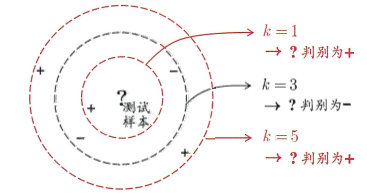
\includegraphics[width=0.4\linewidth]{fig/kNN.png}
\end{figure}

\subsection{主成分分析}
主成分分析(Principle Component Analysis, PCA)

\begin{enumerate}
	\item 对所有样本进行中心化:$\vx_i\gets \vx_i-\frac{1}{m}\sum_{i=1}^m\vx_i$
	\item 计算样本的协方差矩阵$XX^\T$
	\item 对协方差矩阵$XX^\T$做特征值分解
	\item 取最大的$d'$个特征值所对应的特征向量$\vw_1,\vw_2,\ldots,\vw_{d'}$
	\item 输出投影矩阵$W=(\vw_1,\vw_2,\ldots,\vw_{d'})$
\end{enumerate}
